\documentclass{ximera}

\author{Anna Davis} \title{MTH 160 Quiz 24} 

\begin{document}

\begin{abstract}

\end{abstract}
\maketitle
 \textit{Soft Deadline: April 17, 2020}
\begin{problem}\label{prob:quiz23prob1}
For angle $A$ in the triangle shown below, list the exact values of the six trigonometric functions. (Leave square roots in your expressions - do not plug into the calculator.)
\begin{image}
   
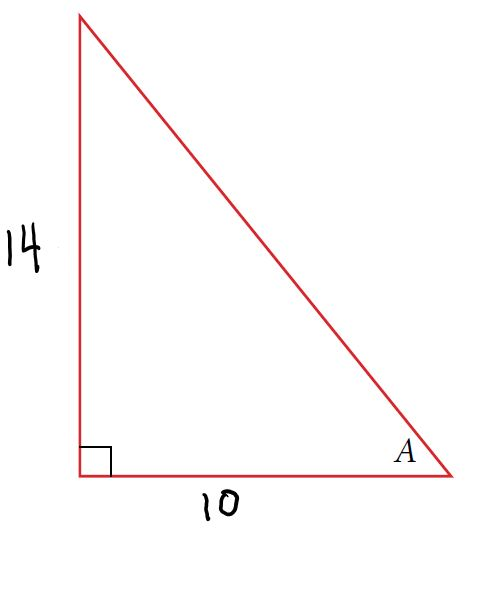
\includegraphics[height=1in]{quiz24image3.jpg}~
 
\end{image}

$$\sin A=\frac{\answer{14}}{\answer{\sqrt{296}}}\quad \csc A=\frac{\answer{\sqrt{296}}}{\answer{14}}$$

$$\cos A=\frac{\answer{10}}{\answer{\sqrt{296}}}\quad \sec A=\frac{\answer{\sqrt{296}}}{\answer{10}}$$

$$\tan A=\frac{\answer{14}}{\answer{10}}\quad \cot A=\frac{\answer{10}}{\answer{14}}$$
\end{problem}

\begin{problem}\label{prob:quiz23prob2}
Solve the triangle.
\begin{image}
   
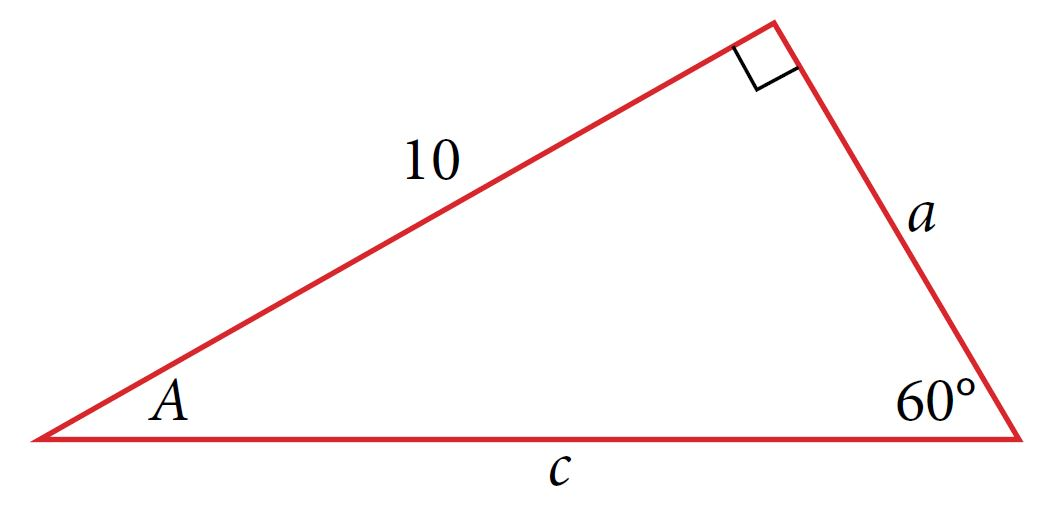
\includegraphics[height=1in]{quiz24image1.jpg}~
 
\end{image}

$$\angle A=\answer{30}\mbox{ degrees}$$
$$a=\answer[tolerance=0.001]{\frac{10}{\sqrt{3}}},\quad c=\answer[tolerance=0.001]{\frac{20}{\sqrt{3}}}$$
\end{problem}

\begin{problem}\label{prob:quiz23prob3}
Solve the triangle.
\begin{image}
   
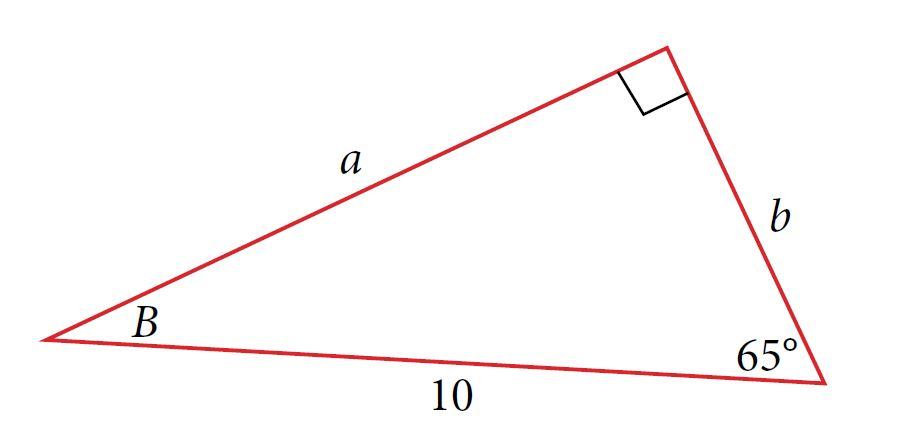
\includegraphics[height=1in]{quiz24image2.jpg}~
 
\end{image}

$$\angle B=\answer{25}\mbox{ degrees}$$
$$a=\answer[tolerance=0.001]{9.063},\quad b=\answer[tolerance=0.001]{4.226}$$
\end{problem}

\end{document} 